\chapter{Requirement Specifications} \label{chap:reqs}

\subsection{Existing System for carpooling}
\justify
Many carpoolings applications and websites have been developed around the world. A similar carpooling system was developed in Massey University New Zealand by a group of students to allow students of Massey University, Albany Campus to share their vehicle with non-vehicle owning students.
\\Following some examples of carpooling systems around the globe : 

\subsection{Websites}
\begin{itemize}

\item New Zealand: https://www.asa.ac.nz/carpool
\item Algeria: www.nroho.com, www.m3aya.com, www.nsogo.net
\item Europe: BlaBlaCar.com, carpooling.com, GoMore.com
\item France: covoiturage.fr
\item USA: car.ma, www.rdvouz.com
\item World: Outpost.travel, joinntravel.com, www.letsride.in

\end{itemize}

\subsection{Mobile Applications}
\begin{itemize}

\item New Zealand: ASA
\item Algeria: YAssir, Nsogo, AMIR
\item World: Uber, sRide, RideShare, 
\item USA: Uber, Lyft
\item France: Karos, Wever, BlaBlaCar, OuiHop

\end{itemize}
\section{Proposed System}
Our purposed system is a “Carpool” application which is a ride sharing application designed just for students. Students can login or signup to this application only via university email id to make sure that only enrolled students in a university used this application.\\

Vehicle owning students can share their rides with other students for traveling to and from their institutes and earn money.

\section{Requirement Specifications}
It involves functional and non-functional functionalities that must be performed by the system:

\subsection{Functional Requirements}

\begin{figure}[ht]
\subsubsection{Functional Requirement - 01}
\centering
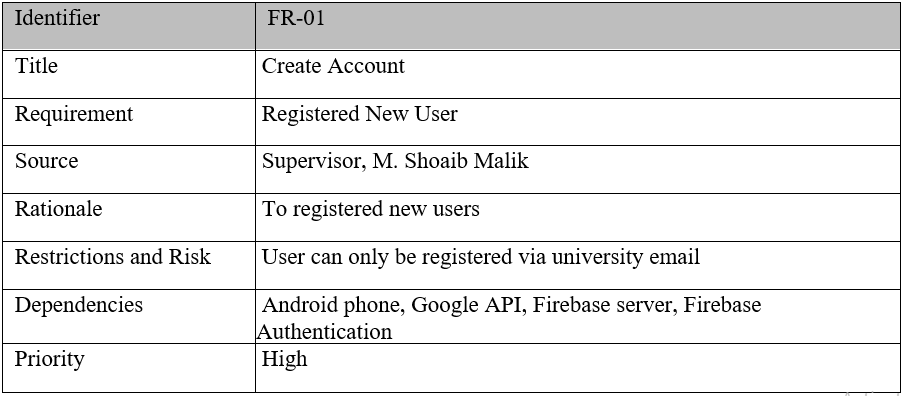
\includegraphics[width=0.8\textwidth]{TableFR1}
\captionof{table}{Functional Requirement - 01}
\end{figure}

\begin{figure}[ht]
\subsubsection{Functional Requirement - 02}
\centering
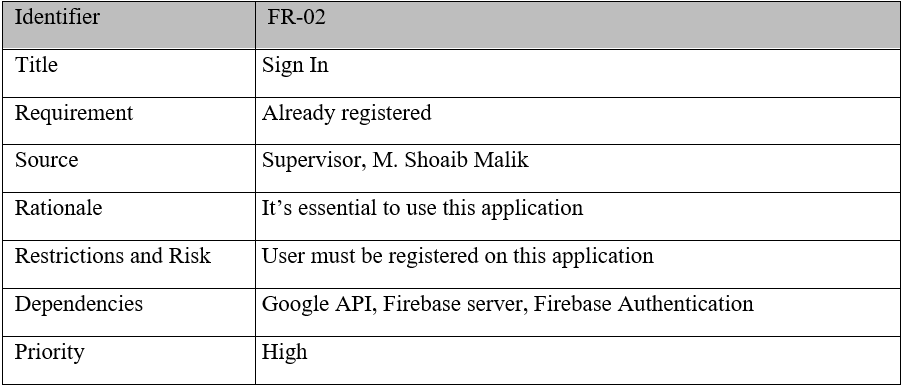
\includegraphics[width=0.8\textwidth]{TableFR2}
\captionof{table}{Functional Requirement - 02}
\end{figure}

\begin{figure}[ht]
\subsubsection{Functional Requirement - 03}
\centering
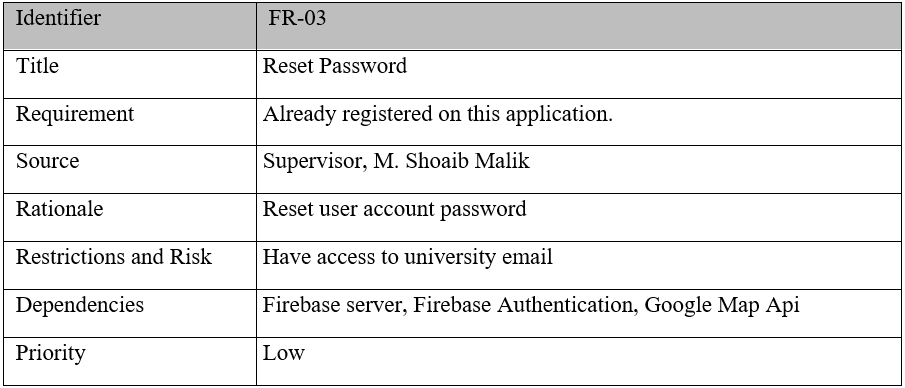
\includegraphics[width=0.8\textwidth]{TableFR3}
\captionof{table}{Functional Requirement - 03}
\end{figure}

\begin{figure}[ht]
\subsubsection{Functional Requirement - 04}
\centering
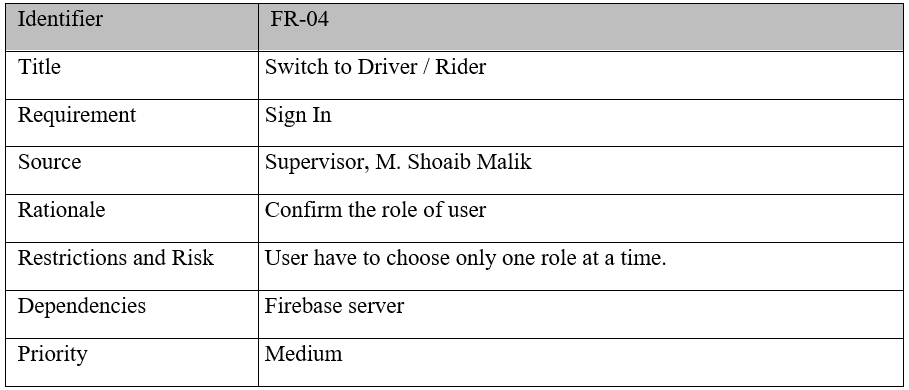
\includegraphics[width=0.8\textwidth]{TableFR4}
\captionof{table}{Functional Requirement - 04}
\end{figure}

\begin{figure}[ht]
\subsubsection{Functional Requirement - 05}
\centering
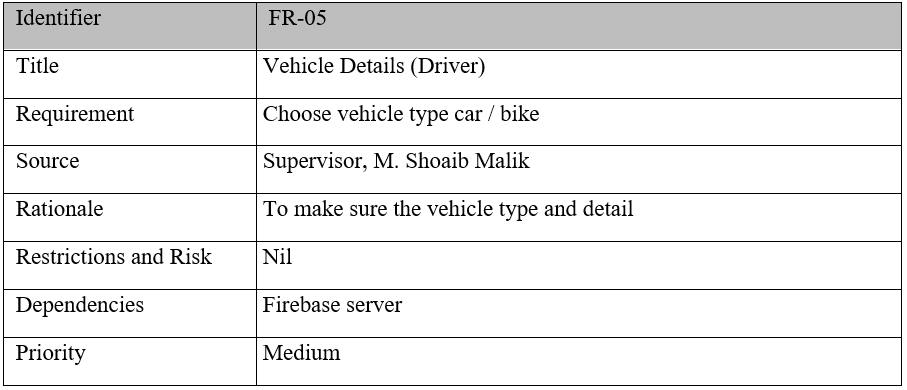
\includegraphics[width=0.8\textwidth]{TableFR5}
\captionof{table}{Functional Requirement - 05}
\end{figure}

\begin{figure}[ht]
\subsubsection{Functional Requirement - 06}
\centering
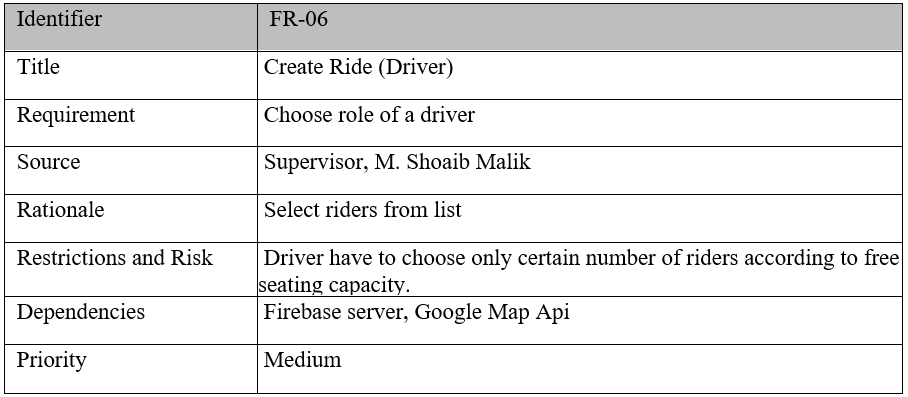
\includegraphics[width=0.8\textwidth]{TableFR6}
\captionof{table}{Functional Requirement - 06}
\end{figure}

\begin{figure}[ht]
\subsubsection{Functional Requirement - 07}
\centering
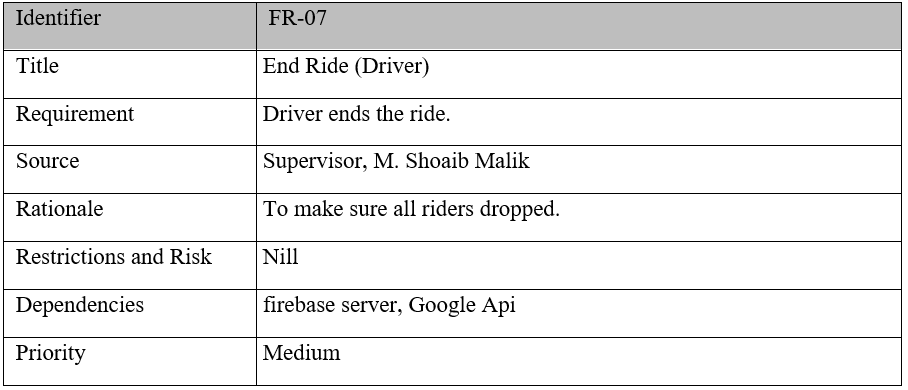
\includegraphics[width=0.8\textwidth]{TableFR7}
\captionof{table}{Functional Requirement - 07}
\end{figure}

\begin{figure}[ht]
\subsubsection{Functional Requirement - 08}
\centering
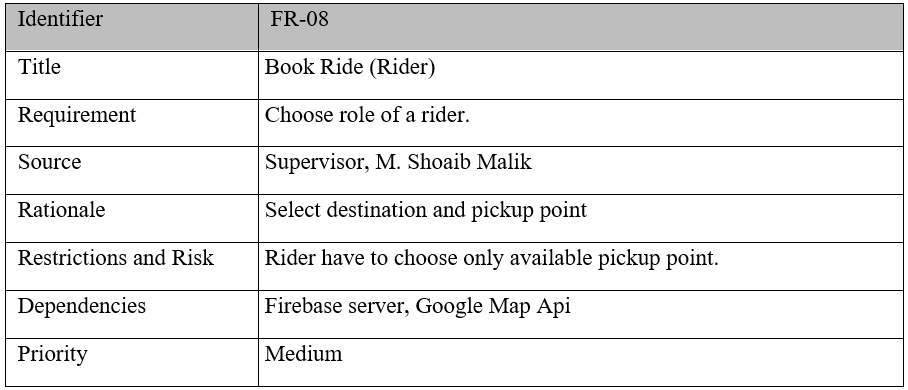
\includegraphics[width=0.8\textwidth]{TableFR8}
\captionof{table}{Functional Requirement - 08}
\end{figure}

\begin{figure}[ht]
\subsubsection{Functional Requirement - 09}
\centering
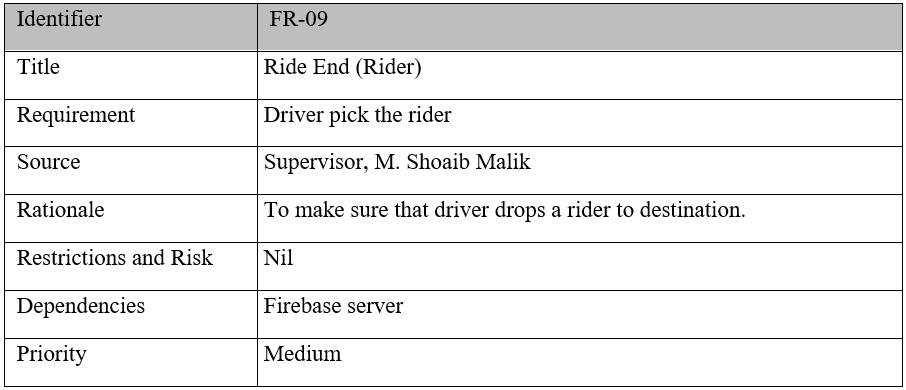
\includegraphics[width=0.8\textwidth]{TableFR9}
\captionof{table}{Functional Requirement - 09}
\end{figure}

\begin{figure}[ht]
\subsection{Non-Functional Requirements} 

\subsubsection{Non-Functional Requirement - 01}
\centering
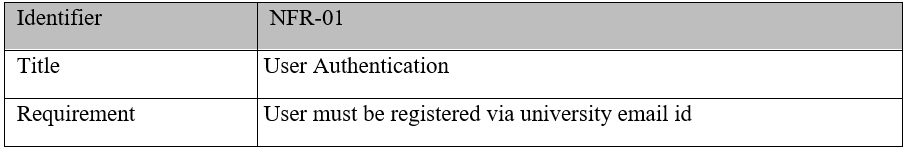
\includegraphics[width=0.8\textwidth]{TableNFR1}
\captionof{table}{Non-Functional Requirement - 01}
\end{figure}

\begin{figure}[ht]
\subsubsection{Non-Functional Requirement - 02}
\centering
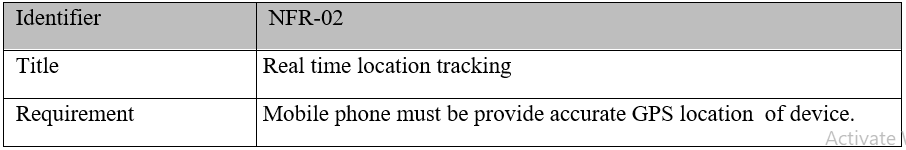
\includegraphics[width=0.8\textwidth]{TableNFR2}
\captionof{table}{Non-Functional Requirement - 02}
\end{figure}

\begin{figure}[ht]
\subsubsection{Non-Functional Requirement - 03}
\centering
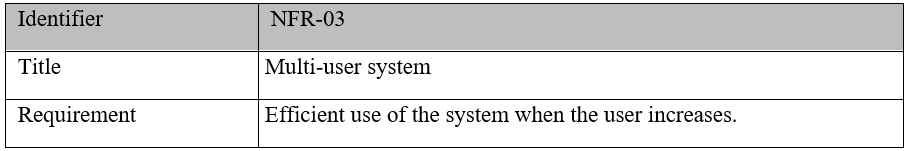
\includegraphics[width=0.8\textwidth]{TableNFR3}
\captionof{table}{Non-Functional Requirement - 03}
\end{figure}

\begin{figure}[ht]
\subsubsection{Non-Functional Requirement - 04}
\centering
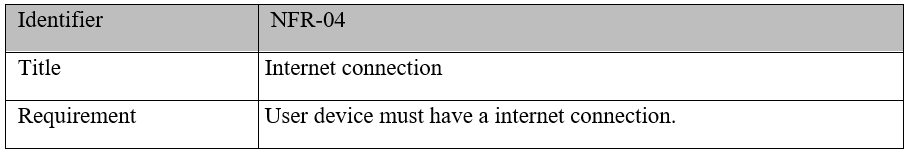
\includegraphics[width=0.8\textwidth]{TableNFR4}
\captionof{table}{Non-Functional Requirement - 04}
\end{figure}

\begin{figure}[ht]
\subsubsection{Non-Functional Requirement - 05}
\centering
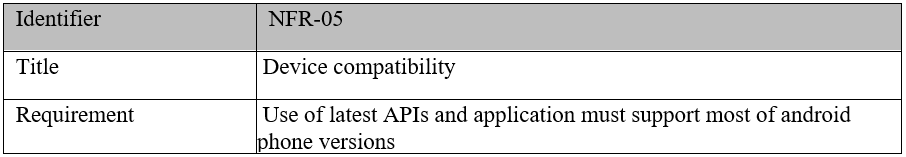
\includegraphics[width=0.8\textwidth]{TableNFR5}
\captionof{table}{Non-Functional Requirement - 05}
\end{figure}

\begin{figure}[ht]
\subsubsection{Non-Functional Requirement - 06}
\centering
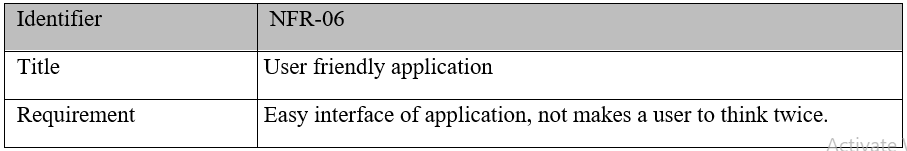
\includegraphics[width=0.8\textwidth]{TableNFR6}
\captionof{table}{Non-Functional Requirement - 06}
\end{figure}

\begin{figure}[ht]
\subsubsection{Non-Functional Requirement - 07}
\centering
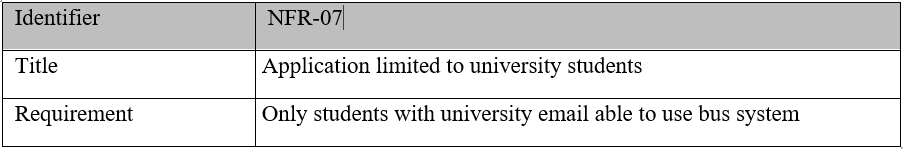
\includegraphics[width=0.8\textwidth]{TableNFR7}
\captionof{table}{Non-Functional Requirement - 07}
\end{figure}
\begin{figure}
\section{Use Cases}
\subsection{Use Case Diagram}
\center
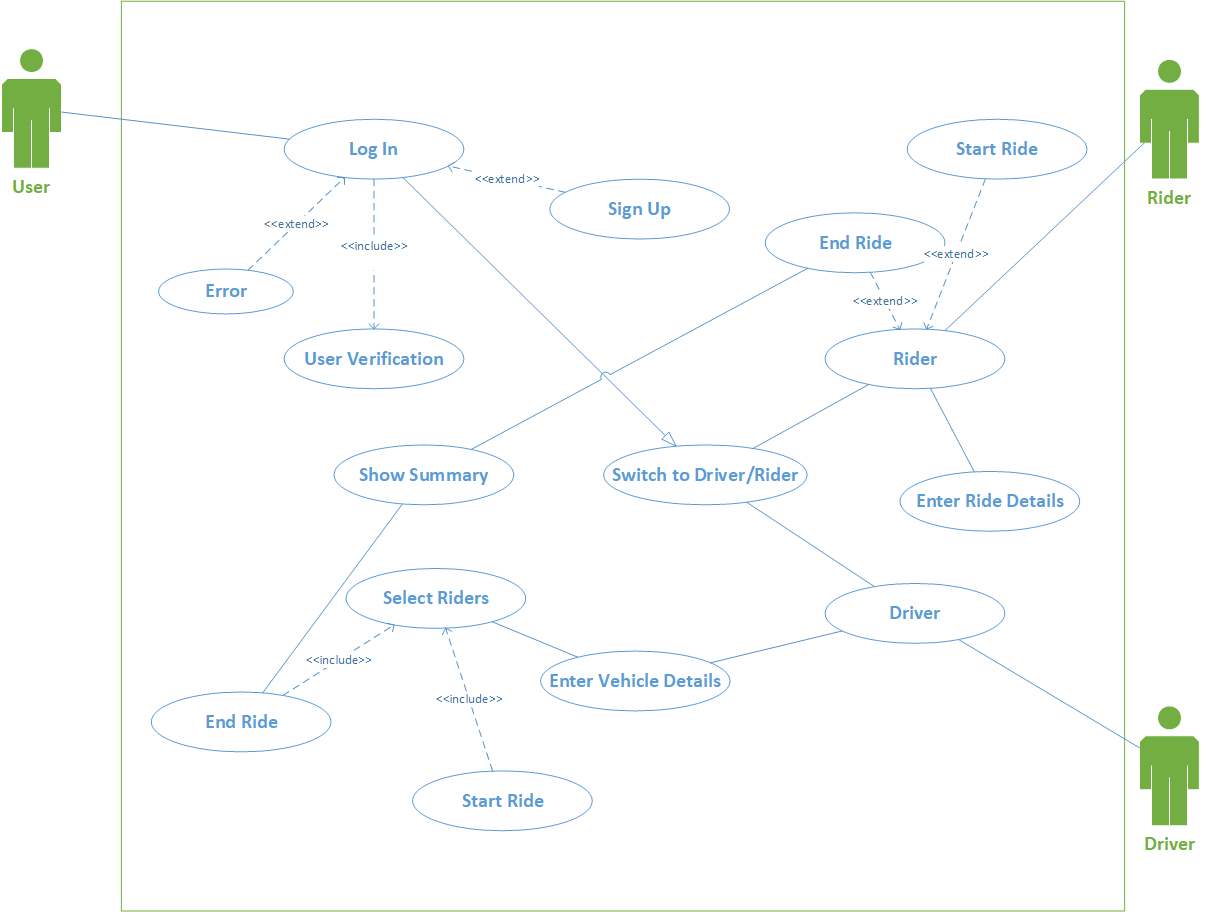
\includegraphics[width=1.0\textwidth]{UseCaseDiagram}
\caption{Use Case Diagram}
\label{fig:UseCaseDiagram}
\end{figure}

\begin{figure}[ht]
\subsection{Use Case Description}
\subsubsection{Table 17: Use Case - 01}
\centering
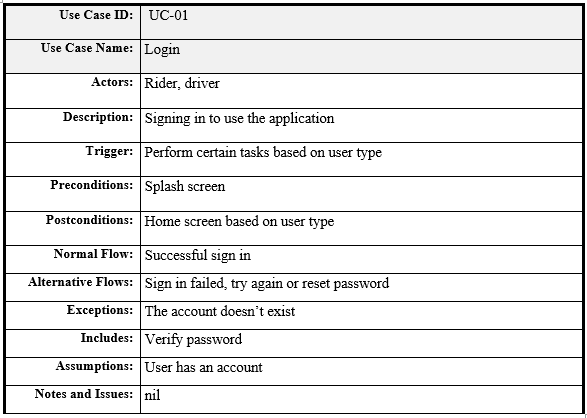
\includegraphics[width=0.8\textwidth]{TableUC1}
\captionof{table}{Use Case - 01}
\end{figure}
\begin{figure}[ht]
\subsubsection{Use Case - 02}
\centering
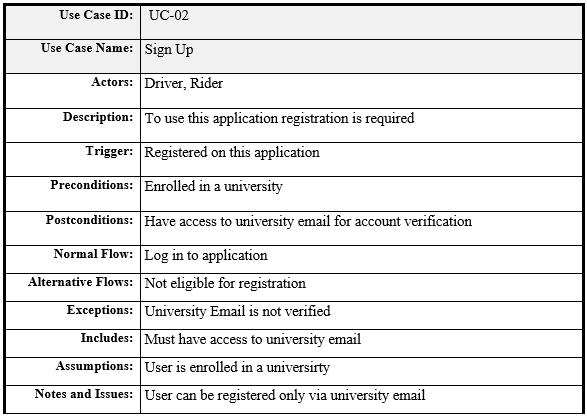
\includegraphics[width=0.8\textwidth]{TableUC2}
\captionof{table}{Use Case - 02}
\end{figure}

\begin{figure}[ht]
\subsubsection{Use Case - 03}
\centering
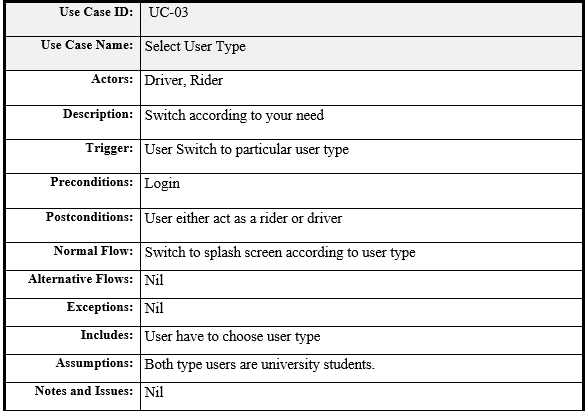
\includegraphics[width=0.8\textwidth]{TableUC3}
\captionof{table}{Use Case - 03}
\end{figure}

\begin{figure}[ht]
\subsubsection{Use Case - 04}
\centering
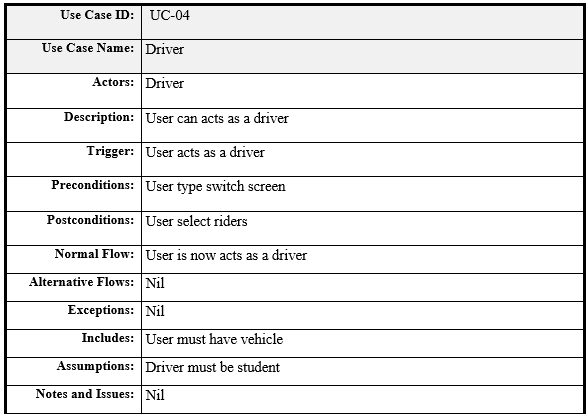
\includegraphics[width=0.8\textwidth]{TableUC4}
\captionof{table}{Use Case - 04}
\end{figure}

\begin{figure}[ht]
\subsubsection{Use Case - 05}
\centering
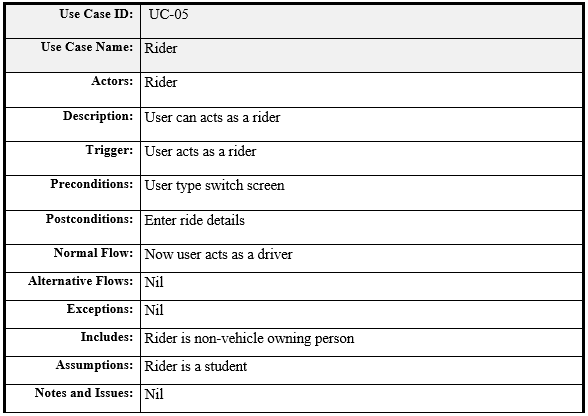
\includegraphics[width=0.8\textwidth]{TableUC5}
\captionof{table}{Use Case - 05}
\end{figure}

\begin{figure}[ht]
\subsubsection{Use Case - 06}
\centering
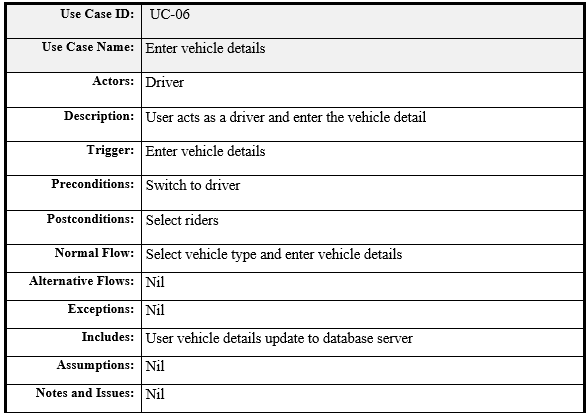
\includegraphics[width=0.8\textwidth]{TableUC6}
\captionof{table}{Use Case - 06}
\end{figure}

\begin{figure}[ht]
\subsubsection{Use Case - 07}
\centering
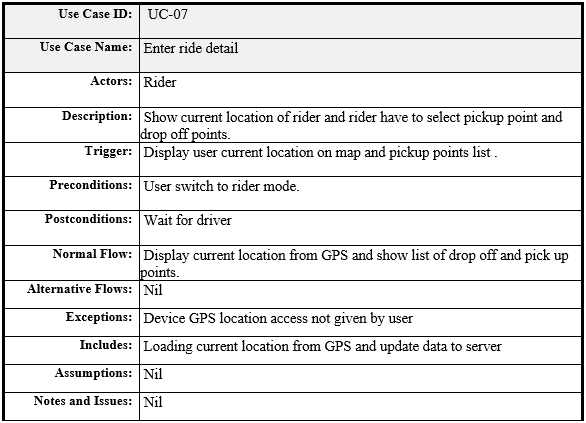
\includegraphics[width=0.8\textwidth]{TableUC7}
\captionof{table}{Use Case - 07}
\end{figure}

\begin{figure}[ht]
\subsubsection{Use Case - 08}
\centering
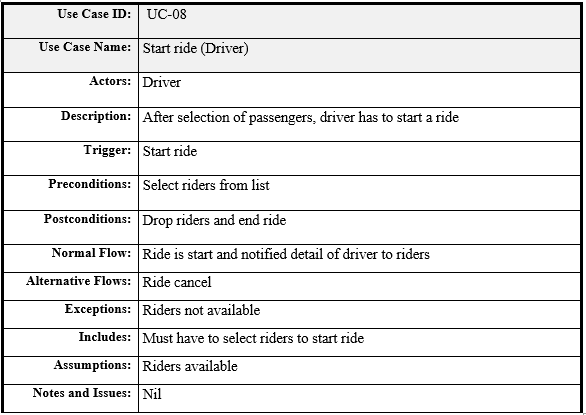
\includegraphics[width=0.8\textwidth]{TableUC8}
\captionof{table}{Use Case - 08}
\end{figure}

\begin{figure}[ht]
\subsubsection{Use Case - 09}
\centering
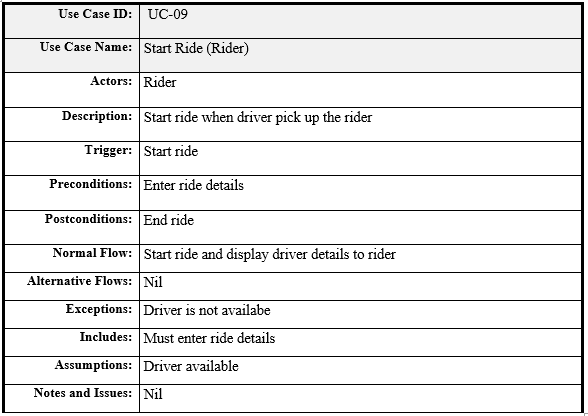
\includegraphics[width=0.8\textwidth]{TableUC9}
\captionof{table}{Use Case - 09}
\end{figure}

\begin{figure}[ht]
\subsubsection{Use Case - 10}
\centering
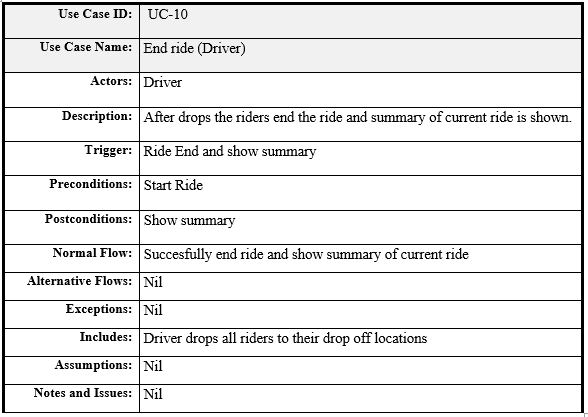
\includegraphics[width=0.8\textwidth]{TableUC10}
\captionof{table}{Use Case - 10}
\end{figure}

\begin{figure}[ht]
\subsubsection{Use Case - 11}
\centering
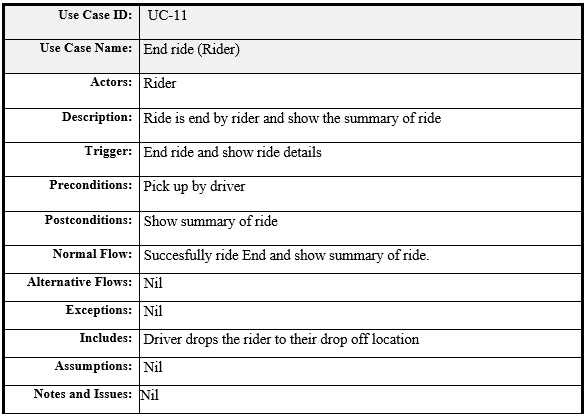
\includegraphics[width=0.8\textwidth]{TableUC11}
\captionof{table}{Use Case - 11}
\end{figure}
 

